\documentclass[a4paper,twoside,11pt]{article}
\usepackage[utf8]{inputenc}
\usepackage[english]{babel}
\usepackage{graphicx}
\usepackage{url}
\usepackage{amsmath}
\usepackage{todonotes}

% redefinição das margens das páginas
\setlength{\textheight}{21.50cm}
\setlength{\textwidth}{15.00cm}
\setlength{\topmargin}{0cm}
\setlength{\headheight}{0cm}
\setlength{\headsep}{0cm}
\setlength{\oddsidemargin}{0.25cm}
\setlength{\evensidemargin}{0.25cm}

% pdflatex

\title{
    \begin{figure}[h]
    \begin{center}
    \resizebox{95mm}{!}{
\includegraphics{logoISEL.png}} 
    \end{center}
    \end{figure}
    \textbf{SVLC: Service virtualization \\into Linux Containers}
}

\author{Daniel Carvalho, A49419@alunos.isel.pt, 913764987 \\}
\date{
    {Supervisors:} \\ 
    {Luis Osório, lo@isel.ipl.pt} \\
    {Mário Pinheiro, mario.pinheiro@isel.pt}\\
    \vspace{5mm}
    March 18, 2024
}

\begin{document}

\maketitle

\section{Introduction}
    The Linux container concept has gained an increasing level of adoption in the last decade, facilitated by the Docker product. The goal for this project is to develop a set of functionalities that facilitate the instantiation, management and deployment of applications or parts of applications (informatics systems of systems) in Linux containers and, as a more advanced objective, in the Kubernetes network. Due to the importance of open standards, the project will adopt open source initiatives, aligned with the Linux Foundation’s Open Container Initiative (OCI).

\section{Background Knowledge}
    In order to understand the reasons and objectives of this project, it is first necessary to know a little more about the themes that are covered in this project.
    
    \subsection{Linux Containers}
        A Linux container is an isolated set of 1 or more processes. All the necessary files are "provided from a distinct image, meaning that Linux  containers are portable and consistent" in all stages of development and production. This also implies a quicker usage when compared with "development pipelines that rely on replicating traditional testing environments"\cite{redhat}.
    
    \subsection{Informatics System of Systems (ISoS)}
        The ISoS is a framework \cite{inproceedings} that proposes an "integration  model to establish a 
        multi-supplier or multi-vendor technology landscape" \cite{inbook}, that works independently from the environment language. 
        An ISoS is composed of one or more \textit{ISystems} that comprises one or more \textit{CES} (Cooperative Enabled Services), which in turn, contains one or more \textit{Services}. 
    
    
\section{Conceptualization of the project}
    This project follows the idea of using ISoS as a starting point to facilitate the development and deployment of Isystems images.
    However, the objective is also to create features that make this process as autonomous as possible. This is achieved by implementing CI/CD (continuous integration and continuous delivery) practices that automate much or all of the manual human intervention traditionally needed to get new code from a commit into production, encompassing the build, test (including integration tests, unit tests, and regression tests), and deploy phases, as well as infrastructure provisioning"\cite{ci/cd}.
    
\section{Technologies}    
    
    For the development of this project we will be using technologies such as:
    
    \begin{enumerate}
        \item Podman/Podman-desktop: To manage and deploy containers\cite{podman};
        \item Quarkus JIB or Eclipse JKube: To programmatically build optimized images for Java applications\cite{quarkusjib}\cite{eclipse};
        \item Kubernets: For distributed deployment, scaling, and management of containerized applications (container orchestrator)\cite{kubernets}.
        \item Visual Paradigm: To create conceptual models in sysml.
        \item Vagrant: For creation and configuration of lightweight, reproducible, and portable development environments\cite{vagrant}.
    \end{enumerate} 
    
\section{Schedule}
    \begin{figure}[h]
    \begin{center}
    \resizebox{130mm}{!}{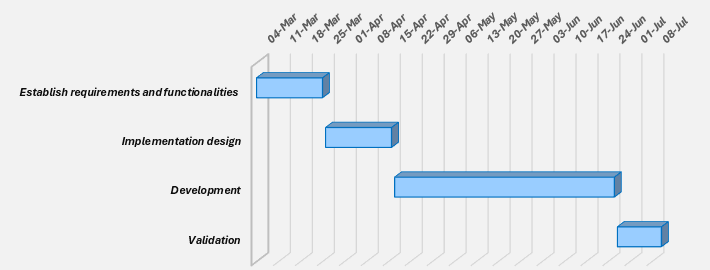
\includegraphics{Schedule.png}}
    \caption{Timeline of each phase of the project (in weeks).}\label{fig:logotipo}
    \end{center}
    \end{figure}

\bibliographystyle{unsrt}
\bibliography{references}

\end{document}